\textbf{Date:} June 5th 2014\\\textbf{Duration:} 9-15\\\textbf{Group
members:} Henrik, Jakob, Jesper

\subsection{Goals for today}

\begin{itemize}
\itemsep1pt\parskip0pt\parsep0pt
\item
  Recognize the intersections
\item
  Get the vehicle to ride the whole track
\end{itemize}

\subsection{Plan}

Do measurements of light values when reaching 4-way intersections and T-intersections from all four directions (there is no T-intersection when northbound).

\subsection{Results}

The way we measured the light values when crossing T intersections is by
enabling the datalogger, and letting the robot follow a line to a T-intersection.
\begin{figure}[hbt]
  \centering
  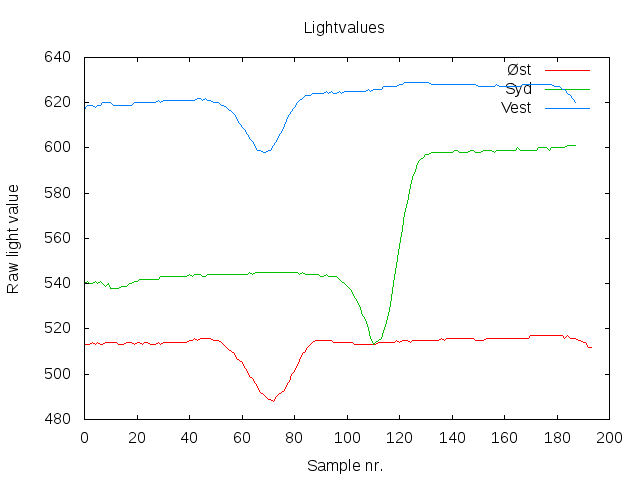
\includegraphics[scale=0.5]{../experiments/2prototype/results/gnuplot/retningsbaseret_3vejs.png}
  \caption{Light values for three different directions when the robot follows a line and see a T-intersection.}
\end{figure}
As
seen in the graph, the offsets are quite different, but the change in
values is very consistent, about 25 units. The "Syd" graph increases after
the intersection, because it entered a white area.\\We tested the same
way for 4-way intersections,
\begin{figure}[hbt]
  \centering
  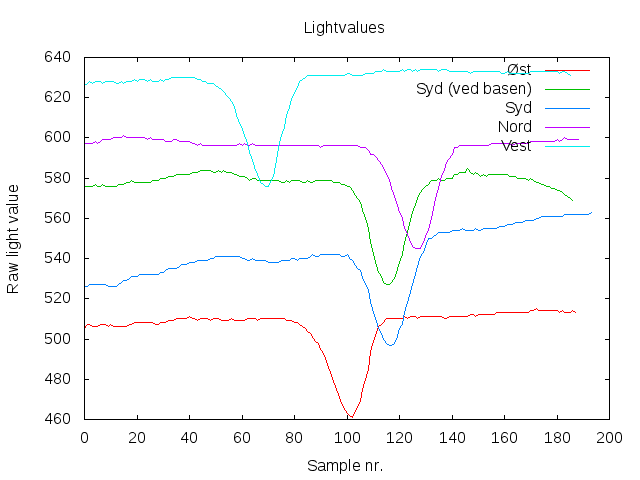
\includegraphics[scale=0.5]{../experiments/2prototype/results/gnuplot/retningsbaseret_4vejs.png}
  \caption{Light values for all four cardinal directions when the robot follows a line and sees a 4-way intersection. South is measured twice due to non-uniform lighting at the track.}
\end{figure}
Again
we see a quite consistent change of values, about 50 units. These tests
show that it is feasible to tell apart T-intersections and 4-way
intersections, although the values are relative to the direction the
vehicle is pointing.

We realized we have not tried driving backwards with the vehicle, so we
tested that.\\\url{http://youtu.be/DYHlgq6TYgY}\\As seen in the video,
it is not possible to drive backwards using the P controller, as the
light sensor is still on the line even though the robot is getting way
off track.

Turns out we need another light sensor in the back if we want to be able
to drive backwards, and so we will attempt one.\\After spending some time
naming variables for light values in a non-confusing manner, we have the second light sensor
installed. The program starts out by calibrating the light sensors, by
driving out into the white area, reading values, turning around, reading
values from another direction, and finally the vehicle starts following
the line towards the solar panels.\\We are now working on getting the
vehicle to follow the track through each line and turn, and once we have
that running, we can use the solar panel manipulation mechanism we
developed last time to finally earn some points.\\We are able to make the
first turn, but we have issues getting the second turn to work. The
light sensor cannot reliably detect the T-intersection, and so it keeps going.
The lighting in the room appears to be the cause of this trouble.\\After
hours of fiddling around with parameters, we found a bug in the code,
and now the vehicle also makes the second turn. We are now well on our
way to the solar panels, so we can finally get some manipulation done!
\url{http://youtu.be/hDwU0r5dlgE}

It turns out the solar panel turning method no longer works accurately, as
our vehicle has been built wider, and the panel is no longer in the
center of it. We had to make adjustments in order to center it again,
and now the vehicle is able to catch a solar panel and rotate it
again.\\The color detection method we wrote yesterday was based on
static lighting conditions, and this is not a feasible solution in
practice. Therefore, we are rewriting it to dynamically calculate the
color thresholds on
runtime.
\begin{figure}[hbt]
  \centering
  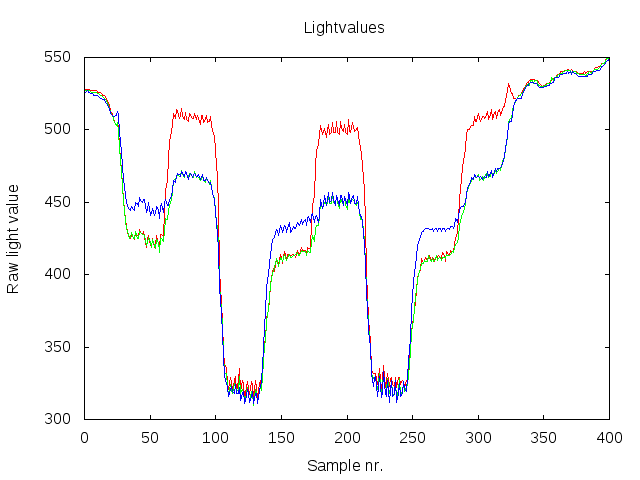
\includegraphics[scale=0.5]{../experiments/2prototype/results/gnuplot/Colormesrun1.png}
  \caption{Color mesurements when the robot drives over 8 solarpannels in a straight line (none,blue,red,black,blue,red,black,blue,red,none)}
\end{figure}

From the RGB value graphs, we see that in order to determine if there is
a panel or not, we only need to look at the blue, or even green, color
value. We will do more research on this next time.

\subsection{Conclusion}

We did not get the vehicle to finish the track today, as we ran into
trouble getting the turns right. Hopefully next time we will get more
turns working, and finish the track. The color sensor still needs some
calibration.
